% Prof. Dr. Ausberto S. Castro Vera
% UENF - CCT - LCMAT - Curso de Ci\^{e}ncia da Computa\c{c}\~{a}o
% Campos, RJ,  2021
% Disciplina: Paradigmas de Linguagens de Programa\c{c}\~{a}o
% Aluno: Javier Ernesto


\chapterimage{img_superior} % Chapter heading image
\chapter{Conclus\~{o}es}
%
%Os problemas enfrentados neste trabalho ...\\
%O trabalho que foi desenvolvido em forma resumida ...\\
%Aspectos n\~{a}o considerados que poderiam ser estudados ou \'{u}teis para ...\\
%   \begin{figure}[H]
%    \begin{center}
%        \caption{Linguagens de programa\c{c}\~{a}o modernas e um bom livro} \label{ling2}
%        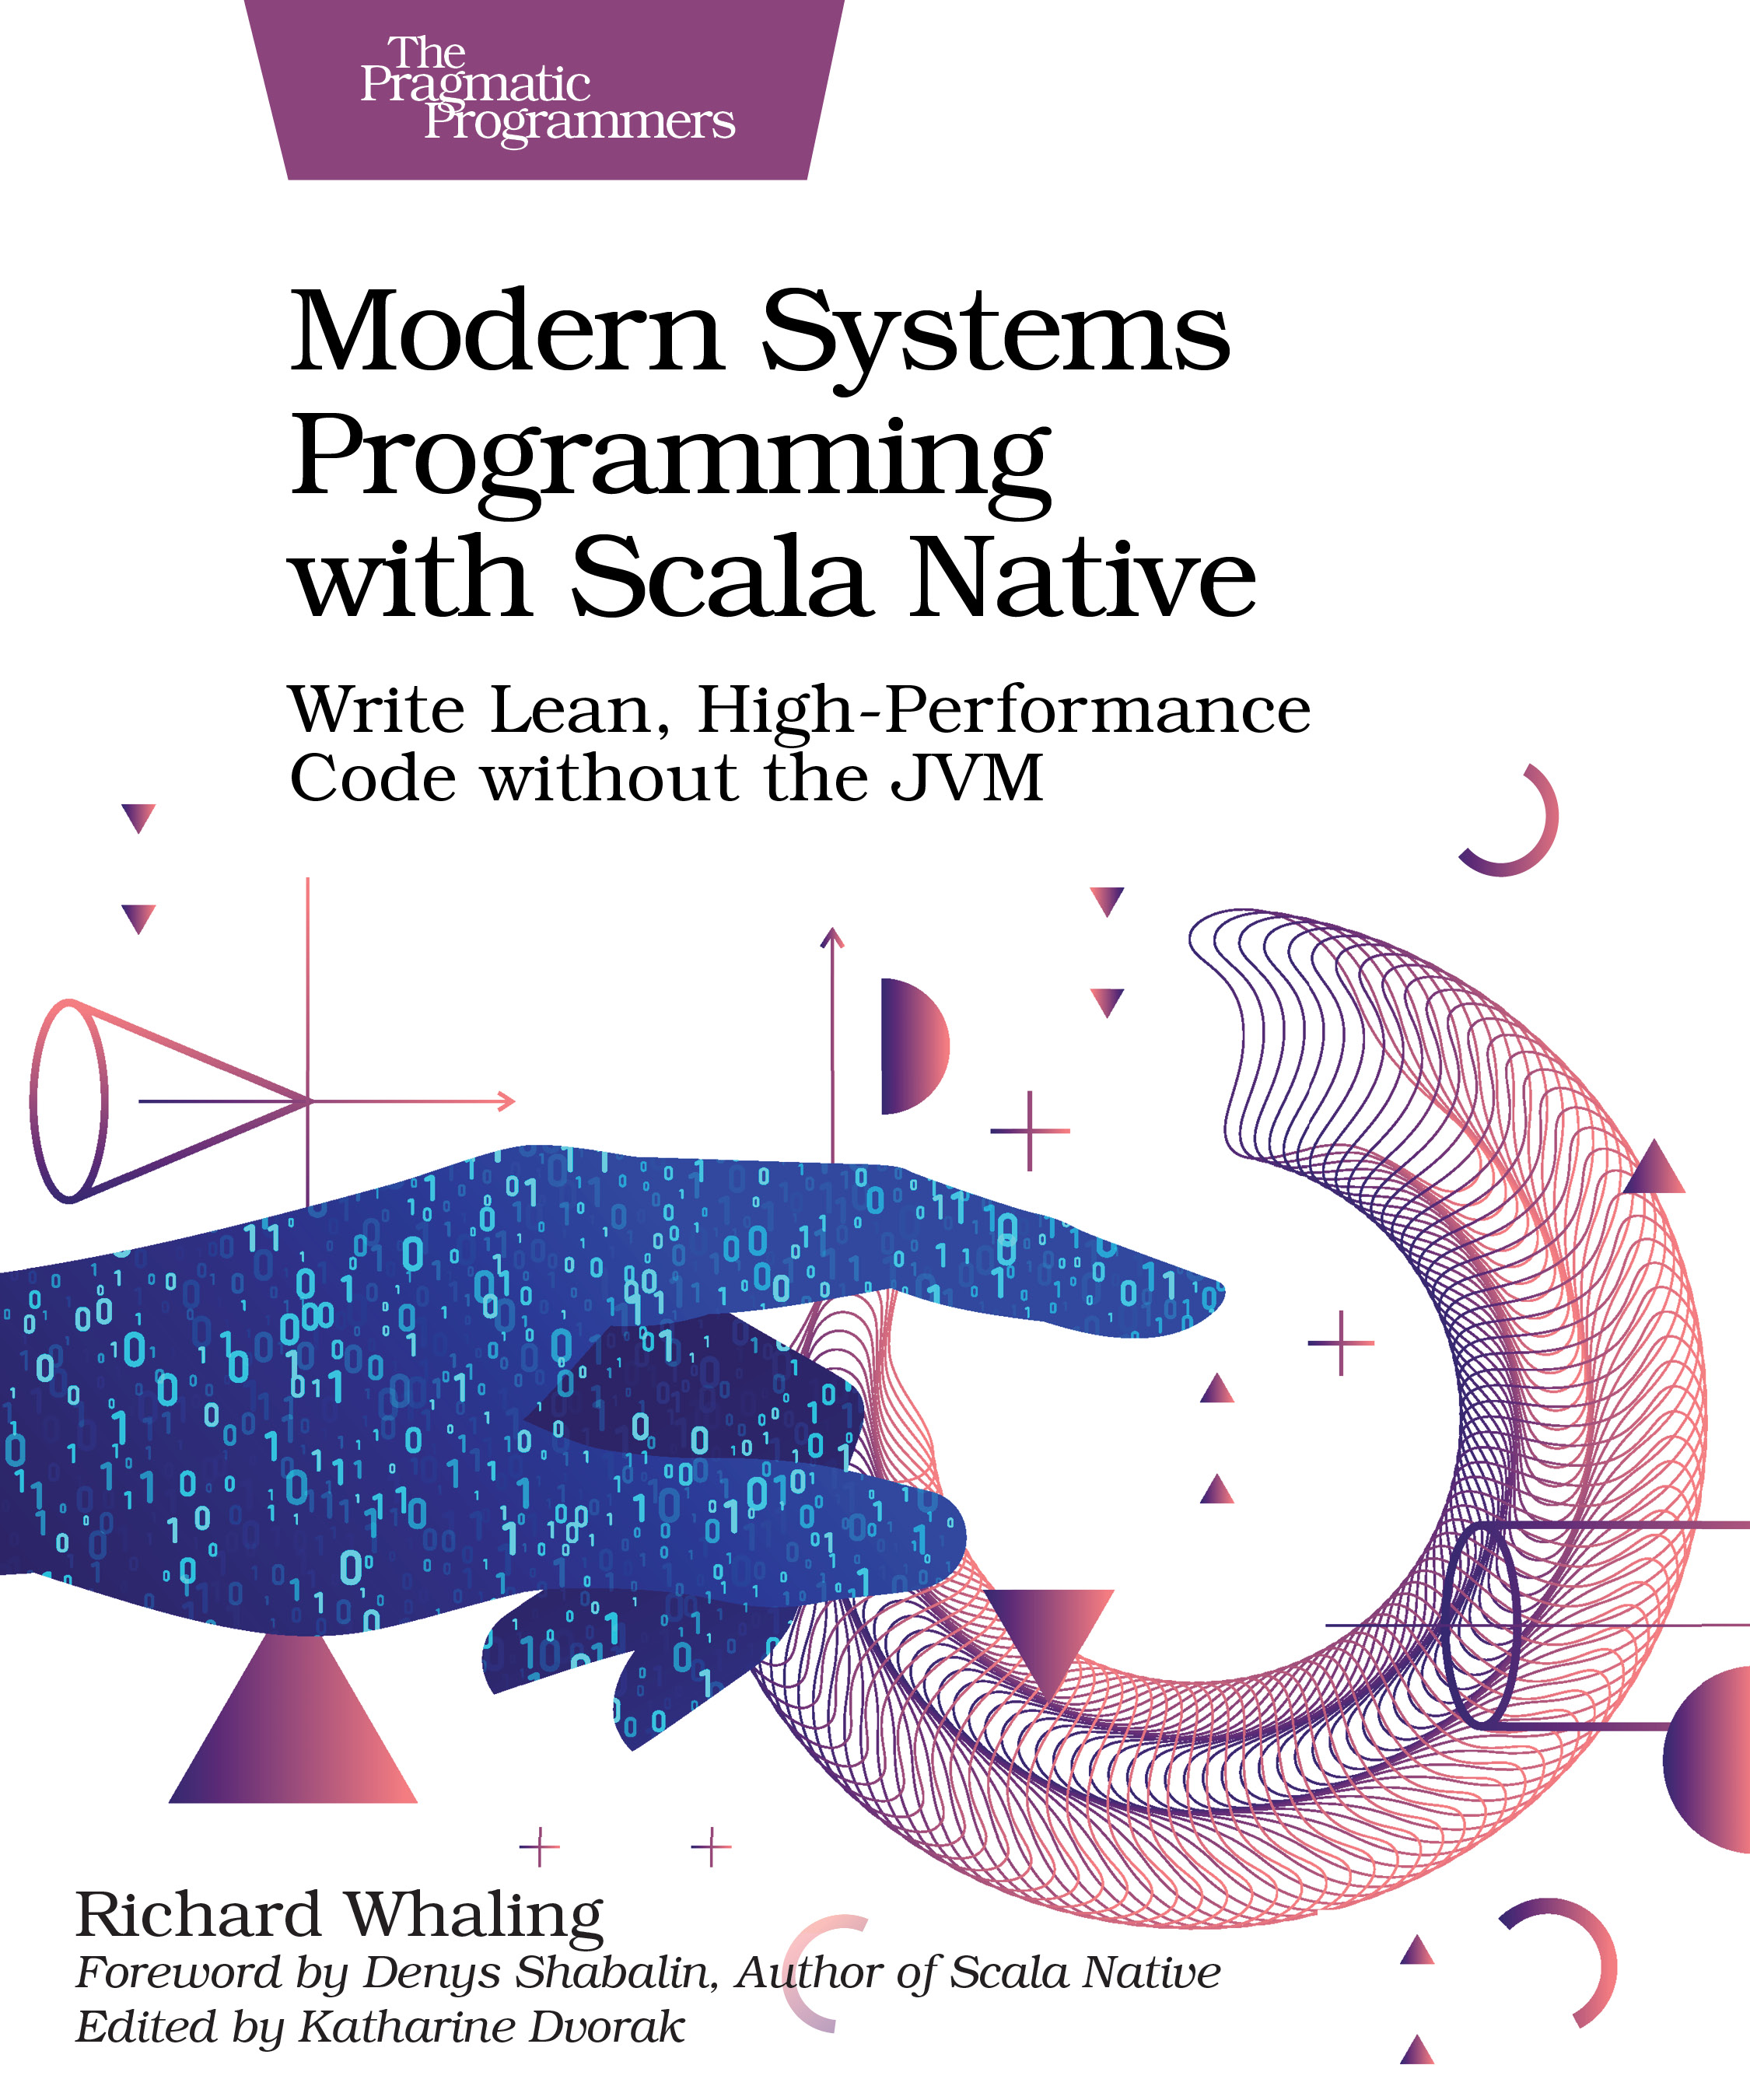
\includegraphics[width=7cm]{livro2020}
%        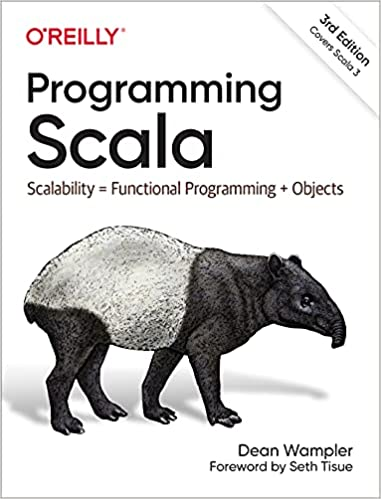
\includegraphics[width=7cm]{livro2021} \\
%        {\tiny \sf Fonte: O autor }
%    \end{center}
%   \end{figure} 